\documentclass[11pt]{article}

\usepackage[letterpaper,margin=0.75in]{geometry}
\usepackage{graphicx}
\usepackage{listings}
\usepackage{subfigure}

\begin{document}

\title{Lab \#1 Report}

\author{Tyler Southwick, Taylor Southwick}

\date{}

\maketitle

\section{Potential Fields}
\subsection{Usage}

We ended up using reflective fields around the obstacles as they seemed to work better than the tangential fields.
At first, we had a guy moving really slow and he followed the fields exactly.
But, as we speed him up, we found that he could get caught in the tangential fields on the four l's world.
By having the walls repulsive with $\beta = 1$ and $s$ equal to the maxDistance from the center of the obstacle to the furthest out edge, making a disk, plus 5 ($s=maxDistance + 5)$ the agent could successfully navigate through the obstacles.

\subsection{four\_ls}

\begin{figure}[h]
	\caption{Potential field towards flag or base}
	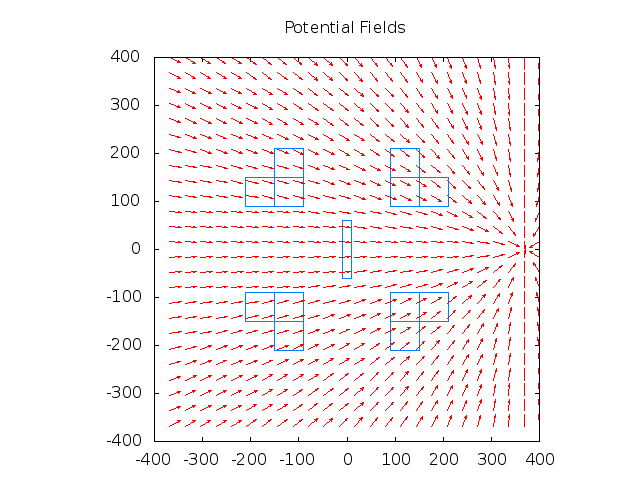
\includegraphics[scale=.2]{plots/four_ls/pfFlag.png}
\end{figure}
\begin{figure}[h]
	\caption{Potential fields away from obstacles}
	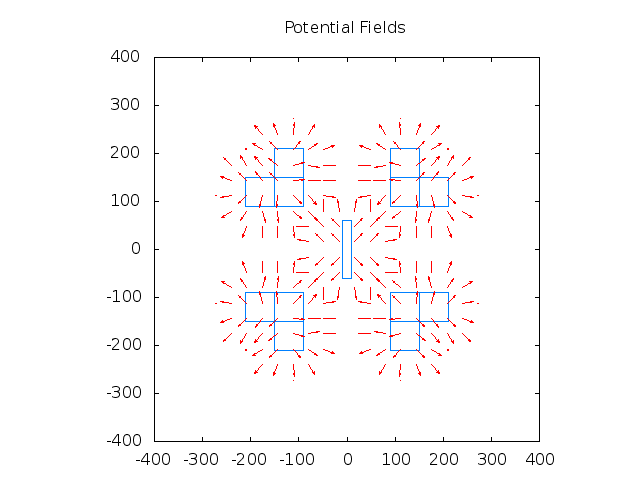
\includegraphics[scale=.2]{plots/four_ls/pfObstacles.png}
\end{figure}
\begin{figure}[h]
	\caption{Potential fields around obstacles (Tangential)}
	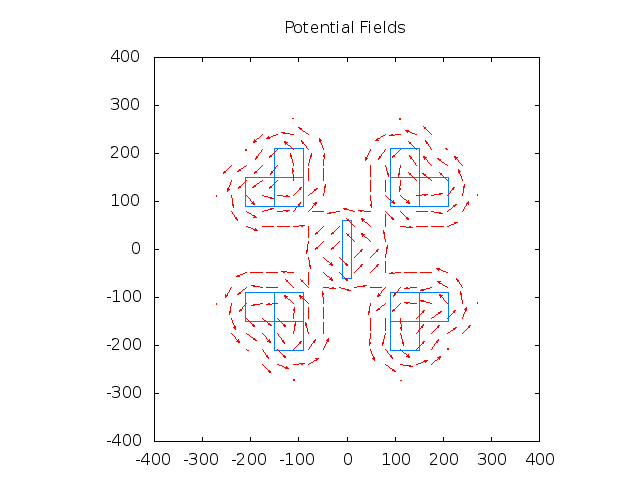
\includegraphics[scale=.2]{plots/four_ls/pfObstaclesTangential.png}
\end{figure}
\begin{figure}[h]
	\caption{Potential field towards flag or base and away from obstacles}
	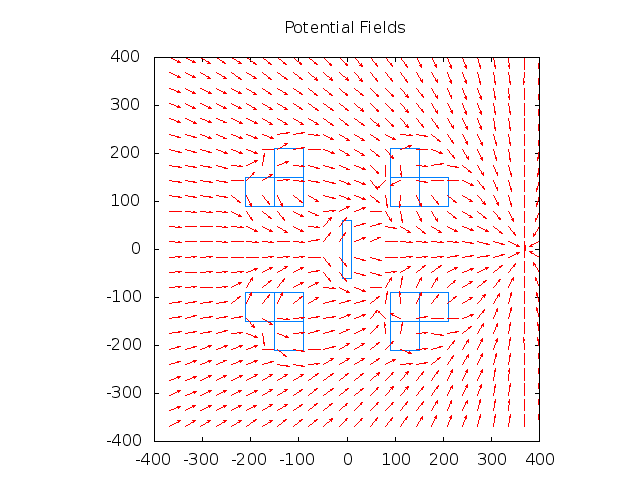
\includegraphics[scale=.2]{plots/four_ls/pfFlagsAndObstacles.png}
\end{figure}

\subsection{rotated squares}

\begin{figure}[h]
	\caption{Potential field towards flag or base}
	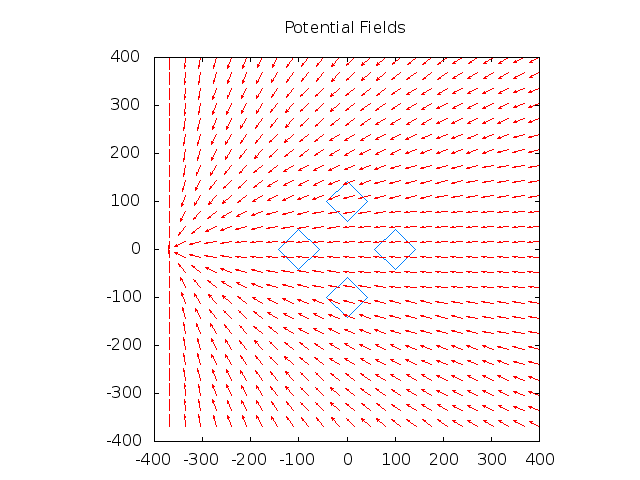
\includegraphics[scale=.2]{plots/rotated_box_world/pfFlag.png}
\end{figure}
\begin{figure}[h]
	\caption{Potential fields away from obstacles}
	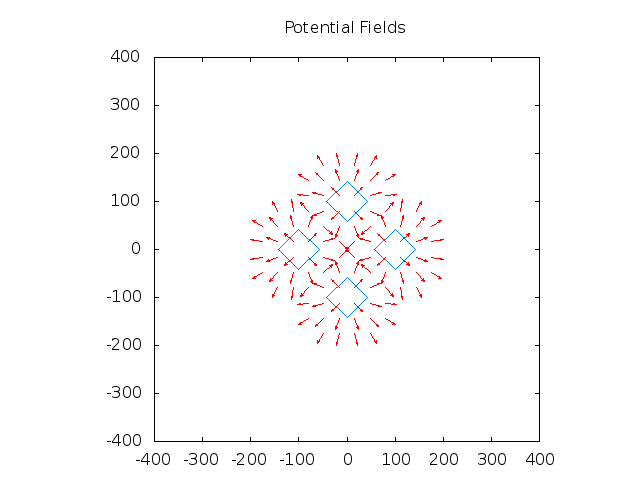
\includegraphics[scale=.2]{plots/rotated_box_world/pfObstacles.png}
\end{figure}
\begin{figure}[h]
	\caption{Potential fields around obstacles (Tangential)}
	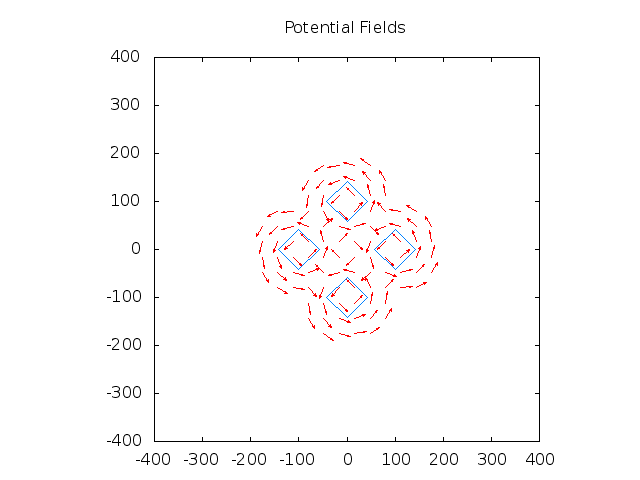
\includegraphics[scale=.2]{plots/rotated_box_world/pfObstaclesTangential.png}
\end{figure}
\begin{figure}[h]
	\caption{Potential field towards flag or base and away from obstacles}
	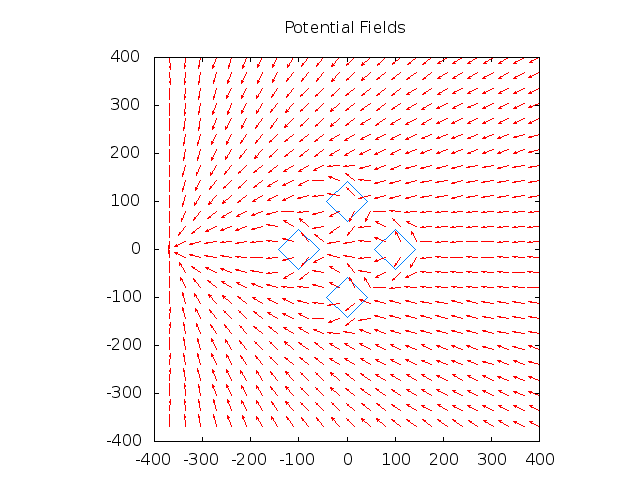
\includegraphics[scale=.2]{plots/rotated_box_world/pfFlagsAndObstacles.png}
\end{figure}

\section{Tests}
We tested our agent against Daniel Brown and Ryan Hintze's agent.
Our PF agent lost against theirs.
We had our PF agent going really slow to guarantee that he followed the field path.
After we ran the tests, we tweaked the values of the different fields as well as our controller and were significantly able to increase speed.

\end{document}
